\chapter[Taggle: A Tag Cloud Visualisation Tool]{Taggle: A Tag Cloud Visualisation Tool}


\label{chap:taggle}
\ifpdf
    \graphicspath{{Chapters/Taggle/TaggleFigs/PNG/}{Chapters/Taggle/TaggleFigs/PDF/}{Chapters/Taggle/TaggleFigs/}}
\else
    \graphicspath{{Chapters/Taggle/TaggleFigs/EPS/}{Chapters/Taggle/TaggleFigs/}}
\fi  

To more effectively support exploration of unknown datasets in software engineering, we designed and
implemented a tag cloud visualisation tool, Taggle, targeted at exploration of software quality assurance metric data. Guided by the design considerations of Chapter~\ref{chap:tagcloud}, the system uses the visual properties of tag clouds to represent data fields, and provides rich interactive features such as dynamic and static filtering to support knowledge discovery. This chapter describes the details of Taggle's implementation; in \S\ref{sect:original} we first discuss the original inherited prototype and changes made in the course of this research. In \S\ref{sect:datamodel} we then review the Taggle data model and describe how data is transformed to fit into this model. Visual encoding used to render the transformed data for display and mapping selection is discussed in the \S\ref{sect:visualencoding}. Finally, in \S\ref{sect:softwaretasks} we present options to complete a set of software engineering tasks using Taggle.

\section{Original prototype}\label{sect:original}

An interactive tag cloud visualisation tool implemented using the Java 2D API was inherited from previous University of Canterbury research. Some aspects of the original prototype are shown in Figure~\vref{fig:original} and descriptions can be found in technical documents: \citet{deaker11, deaker11b, deaker11c}.

\begin{figure}[!htb]
\centering
\begin{subfigure}{.5\textwidth}
  \centering
  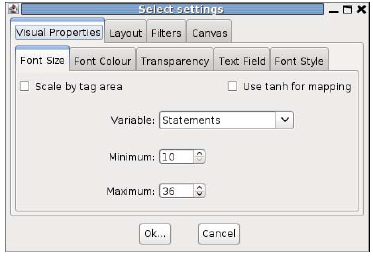
\includegraphics[scale=0.50]{old1.png}
  \caption{Mapping selection font size}
\end{subfigure}%
\begin{subfigure}{.5\textwidth}
  \centering
  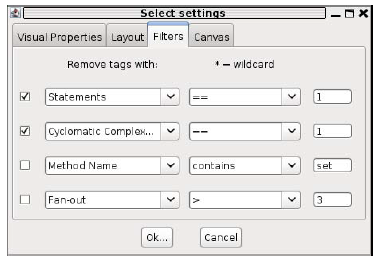
\includegraphics[scale=0.50]{old2.png}
  \caption{Tag filtering}
\end{subfigure}
\begin{subfigure}{\textwidth}
  \centering
  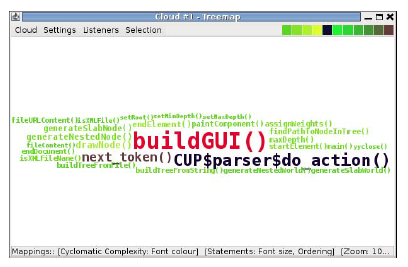
\includegraphics[scale=0.80]{old3.png}
  \caption{Canvas with tag cloud and colour chip legend}
\end{subfigure}%
\caption{\textit{Original Taggle prototype}}
\label{fig:original}
\end{figure}

In this research, I have extended and enhanced this prototype in order to create a stable system which could satisfactorily explore software quality assurance data such as metrics and code smells using tag cloud visualisation. Additionally, the possibility of using other software artefacts such as process management data and general multi-variate data, has been left open.

In the course of this research, changes were made to the original prototype which included:

\begin{itemize}
\item implementation of changes resulting from software engineering challenges and tag cloud visual variable analysis (Chapter~\ref{chap:tagcloud})
\item improvements generated from heuristic evaluation (Chapter~\ref{chap:heuristiceval})
\item implementation of an XML data conversion utility 
\item usability improvements and bug fixes
\end{itemize}

The software pictured and described in the rest of this chapter refer to the final prototype, after all alterations and improvements have been made.

\section{Data model and transformation}\label{sect:datamodel}

Source data for Taggle may be generated externally and provided in an XML format conforming to a DTD. There are a variety of tools/methods which can produce software metric data from static analysis of source code (such as that proposed by \citet{irwin03}, and see Appendix~\ref{appdx:tools} for a list of available plugins, software analysis platforms and frameworks/tools that can generate metric data). Most of these tools can output data into a CSV or XML format (\S\ref{sect:met}). I produced a tool to convert CSV formatted data to the Taggle XML format. This has also proved useful for conversion of datasets that may easily be obtained from external sources such as \url{www.findthedata.com}. Tools which produce XML formatted output only may also be transformed (using XSLT for example). 

The Taggle XML format specifies such things as measurement scales (nominal, ordinal and ratio) and relationships. Datasets consist of records (data points), each containing a number of fields. Visual mappings to properties and constraints for each data field can be specified via the GUI. Once the constraints of the visual property are set, a relative weighting for each tag is calculated according to the rank of the measurement. The calculation of rank is dependent on the measurement scale type. The weightings are used to calculate the value of the visual property for an individual tag, between the user defined constraints for a visual property (for example minimum and maximum font sizes). A full description of the Taggle XML format and weighting calculations can be found in \citet{deaker11c}.

As an example, consider the tag cloud in Figure~\vref{fig:activemqcamel}: the XML source file contained quality metrics from a subproject of open source project  ActiveMQ, the metrics were of the Chidamber and Kemerer suite generated by the CKJM toolkit. These were originally produced in space-separated text format, converted to CSV by OpenOffice, and then converted to the Taggle XML format by our conversion tool. In the GUI, the nominal field ``Class'' was mapped to the tag text (Arial font), the ratio field ``LCOM'' was mapped to the tag ordering property and the font size property (spanning from 20pt to 35pt), and the ratio field ``CBO'' was mapped to a background colour range from black to red. The tags have been positioned according to a simple tag cloud layout algorithm ``typewriter'', where the tags are mapped sequentially left to right, top to bottom (ways to improve the overall presentation are discussed later in the chapter). Default values for the visual mappings and other settings for Taggle can be controlled using an external XML file. 

\begin{figure}[!htb]
  	\centering
   	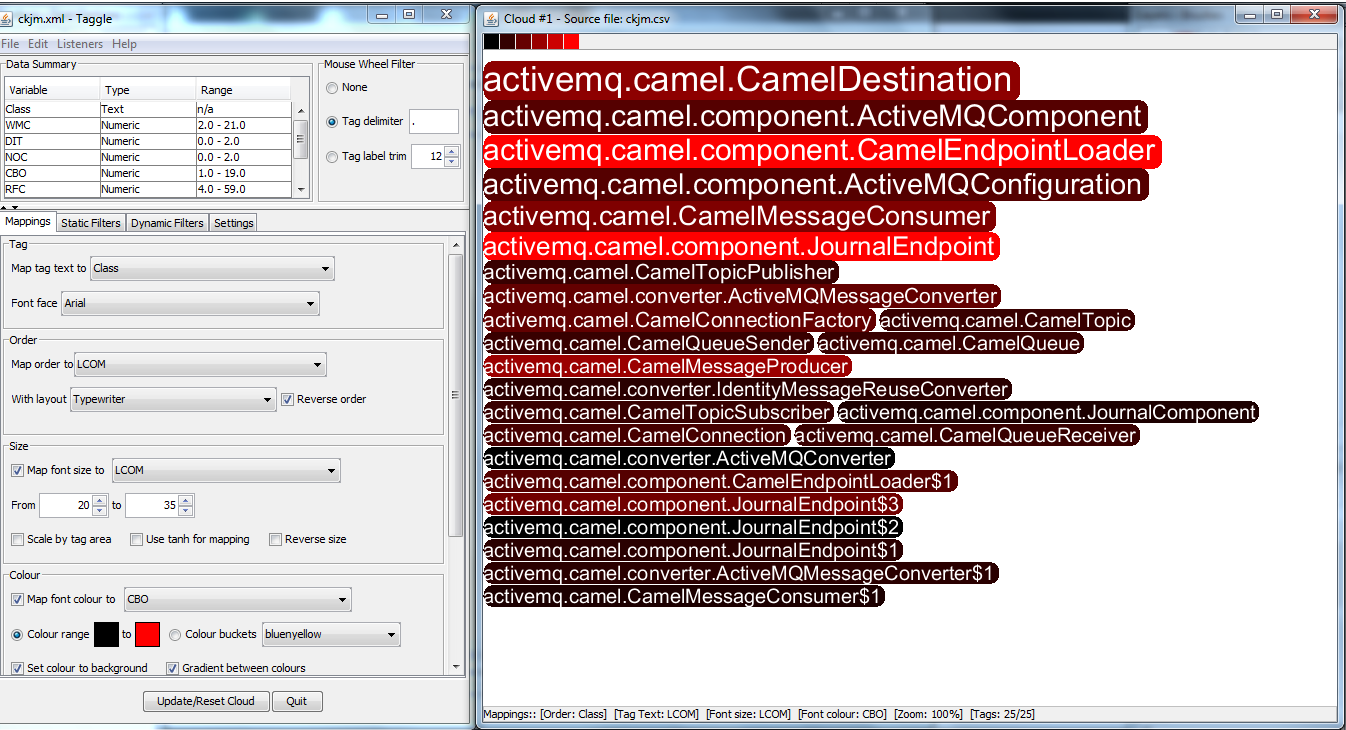
\includegraphics{activemqcamel.png}
  	\caption{\textit{A tag cloud generated by Taggle depicting a subproject of ActiveMQ with metrics derived from CKJM. Visual mapping interface is on the left.}}
	\label{fig:activemqcamel}
\end{figure}

\section{Visual encoding and mapping selection}\label{sect:visualencoding}

For brevity, only visual encoding and mapping features utilised in this research are discussed in this section. Information regarding other mapping properties and tag cloud layout algorithms can be found in the following technical documents: \citet{deaker11, deaker11c} (note that these documents describe the basic procedure which hasn't changed much, whereas the graphical interface, numbers of options, and features have changed significantly through the course of this research).

The mapping selection interface can be seen in Figure~\vref{fig:mappingselection}. In the analysis of visual properties available in tag clouds (Chapter~\ref{chap:tagcloud}), order, size, colour and transparency were deemed the most appropriate visual variables for data mapping purposes. The order in which they are displayed on the central mapping pane is in order of perceived usefulness and importance (with tag order being the most useful and transparency the least useful). By default, only the minimum mappings essential for display (tag and tag order) are turned on.

\begin{figure}[!htb]
\begin{subfigure}{.5\textwidth}
	\centering
	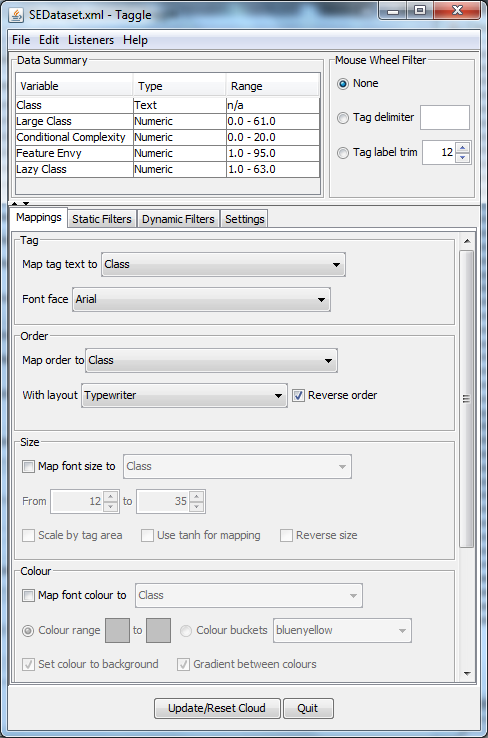
\includegraphics[scale=0.40]{mappings1.png}
	\caption{\textit{Data summary panel toggled on}}
\end{subfigure}%
\begin{subfigure}{.5\textwidth}
  \centering
  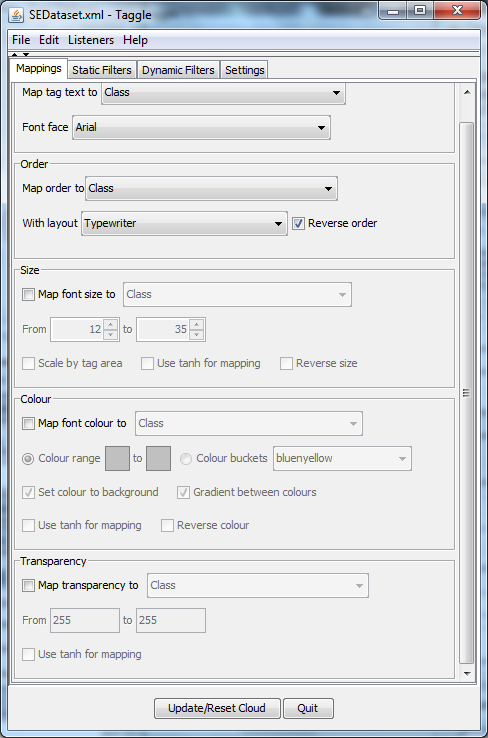
\includegraphics[scale=0.40]{mappings2.png}
  \caption{\textit{Data summary panel toggled off}}
\end{subfigure}
  \caption{\textit{Mapping selection interface: the data summary panel can be toggled by the user as desired to save valuable screen space}}
  \label{fig:mappingselection}
\end{figure}

The user is supported in the choice of appropriate mappings for the tag cloud by a data summary screen shown in a resizeable pane at the top of the GUI --- for an example see Figure~\vref{fig:datasummary}. Each field in the data file is shown along with data type (text, numeric or categorical) and the range of values in the category.  The data summary panel was included by request from a heuristic evaluation (see Chapter~\ref{chap:heuristiceval}).

\begin{figure}[!htb]
  	\centering
   	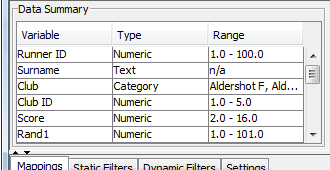
\includegraphics[scale=0.80]{datasummary2.png}
  	\caption{\textit{Closeup of an example data summary panel}}
	\label{fig:datasummary}
\end{figure}

\subsection{Categorical and continuous data}

Data types displayed in the data summary screen are determined programmatically. Fields are labelled categorical when the value ranges correspond to a certain maximum distinct number of values (the actual number is controlled via a setting). It is limited to a particular number of distinct values to match the number of colour chips displayed in the legend --- categorical variables are used predominantly in display colour mappings (\S\ref{colourmappings}). Providing a method for distinguishing these two types of data was included by request from the heuristic evaluation, where it was determined to be useful to display categorical data using a unique colour for each category.

\subsection{Tag}

\paragraph{Visual variable: tag length} The user is free to select any field to map to the tag text, including numeric types. The tag lengths for each tag will differ depending on the number of characters in the tag text. To minimise the possible effects on perception long textual identifiers may have, see \S\ref{sect:textualdata} for a description of the application of filters.

\paragraph{Visual variable: font family} The font face dropdown box is pre-populated with fonts that are installed on the machine running Taggle. Because reading ease is improved when presented with familiar fonts \citep[pg 106, chap 11:7][]{usability06}, Arial, Helvetica and Times New Roman (or the equivalents depending on the operating system and installed word processing software) are presented for selection at the top of the dropdown box, separated by a divider (see Figure~\vref{fig:fontfamily}).

\begin{figure}[!htb]
  	\centering
   	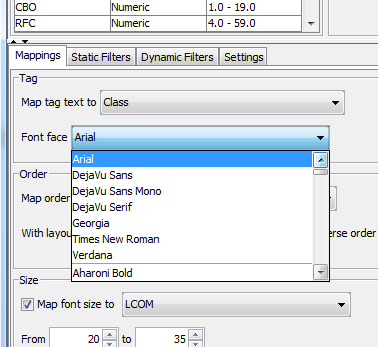
\includegraphics[scale=0.50]{fontfamily.png}
  	\caption{\textit{Prompting selection of familiar fonts.}}
	\label{fig:fontfamily}
\end{figure}

\subsection{Order}

\paragraph{Visual variable: order} If the order visual property is mapped to a field containing textual data, ordering of the tags is determined alphabetically, otherwise tags are ranked by their numerical value. The selected ordering can be reversed with the ``reverse order'' checkbox and updating the tag cloud. The user can select an appropriate layout from typewriter, spiral or force directed (defaulting to the simplest layout, typewriter).

\subsection{Size}

\paragraph{Visual variable: font size} Research has indicated slower reading performance for smaller font size \citep[pg 107, chap 11:8][]{usability06}, so there are constraints on the minimum font size to be set to no less than 9pt. The maximum font size is constrained to 250pt: by default this is set to a much smaller 35pt to allow for a smaller screen and canvas size (canvas size can be adjusted from the settings tab). The data mapped to the selected font sizes can be reversed with the ``reverse size'' checkbox.

\subsection{Colour and transparency} \label{colourmappings}

\paragraph{Visual variable: background colour} The heuristic evaluation and controlled experiments conducted in this research determined that the use of background colour was useful for visual search with colour mappings, as well as dataset features such as multiple word tags. Background colour has also been found to support more accurate estimation of relevant tags \citep{waldner13}. Therefore tag display via background colour is the default setting in Taggle. 

The user may select from a choice of colour range (between user defined colours) or colour buckets (a set palette of colours) --- see Figure~\vref{fig:colourinterface}. When the user chooses a data field to map to colour, colour range or colour bucket is automatically selected depending on whether the data field is categorical data. Categorical data is best displayed through a unique set of colours preselected from a colour palette (the colour palettes can be user defined through external string property files, although default palettes are provided.) For example, in Figure~\vref{fig:colourbuckets} a dataset about agile projects is displayed in a tag cloud. With the aim of finding what actors are related to the agile stories with the highest time estimates, order/size are mapped to estimate and colour is mapped to actor. The user can determine stories with the greatest estimated workload corresponding to tags coloured dark grey and brown, and find details via a colour legend mouse hover or tag label mouse hover (actors `Preferred customer' or `Bookstore customer').

Continuous data is best displayed through a colour range. The user has the option of choosing a colour gradient between two selected colours, or colours which appear on the colour wheel between two selected colours (see Figure~\vref{fig:continuous}. Colour models are complicated and won't be discussed in full detail). Like other mappings, the user also has the option to reverse the selected mappings so high values can be shown with the `from' colour and low values can be shown with the `to' colour.

\begin{figure}[!htb]
  	\centering
   	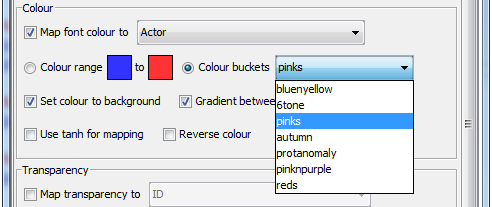
\includegraphics[scale=0.75]{colourinterface.png}
  	\caption{\textit{Colour mapping interface}}
	\label{fig:colourinterface}
\end{figure}

\begin{figure}[!htb]
\begin{subfigure}{.5\textwidth}
	\centering
	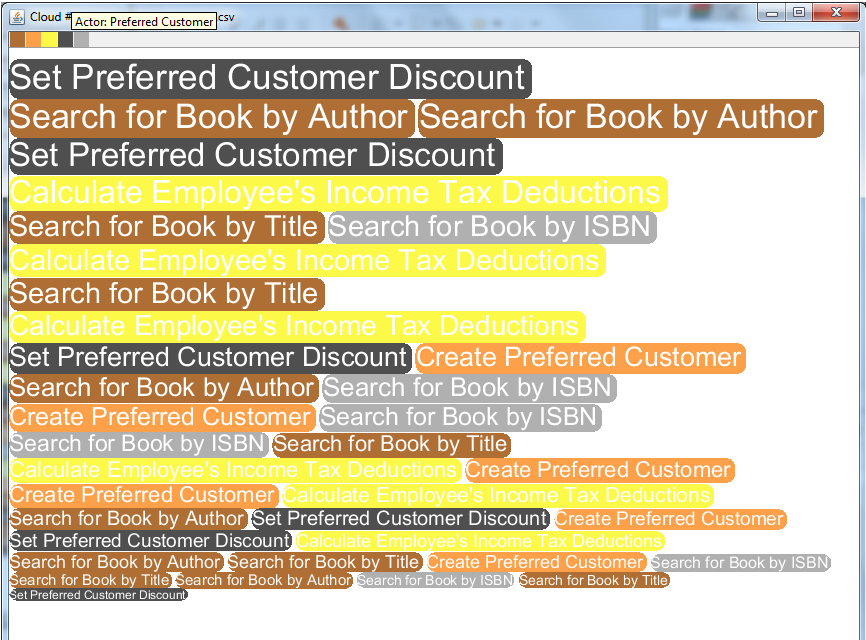
\includegraphics[scale=0.20]{colourbuckets1.png}
	\caption{\textit{Mouse over the legend}}
\end{subfigure}%
\begin{subfigure}{.5\textwidth}
  \centering
  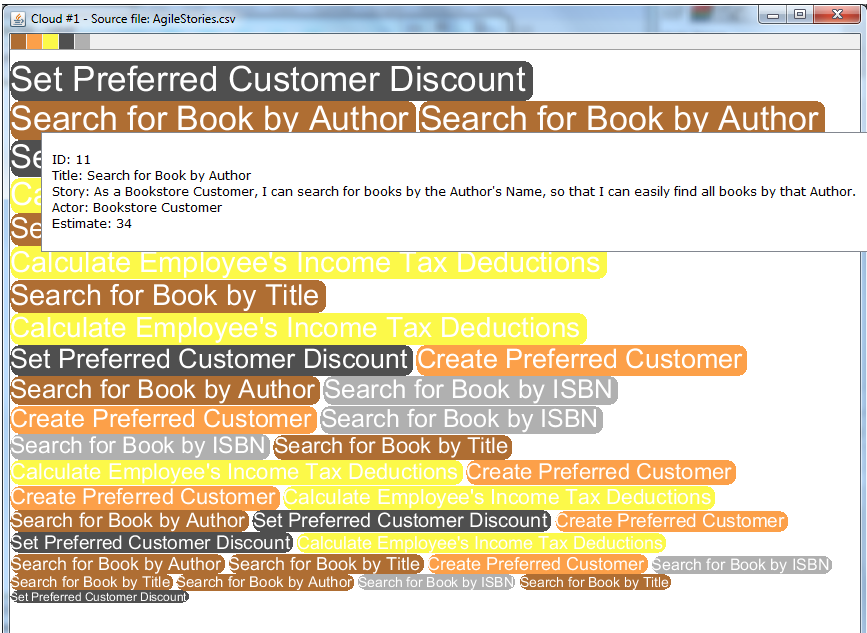
\includegraphics[scale=0.20]{colourbuckets2.png}
  \caption{\textit{Mouse over a tag}}
\end{subfigure}
  \caption{\textit{Displaying categorical data with colour buckets}}
  \label{fig:colourbuckets}
\end{figure}

\begin{figure}[!htb]
\begin{subfigure}{.5\textwidth}
	\centering
	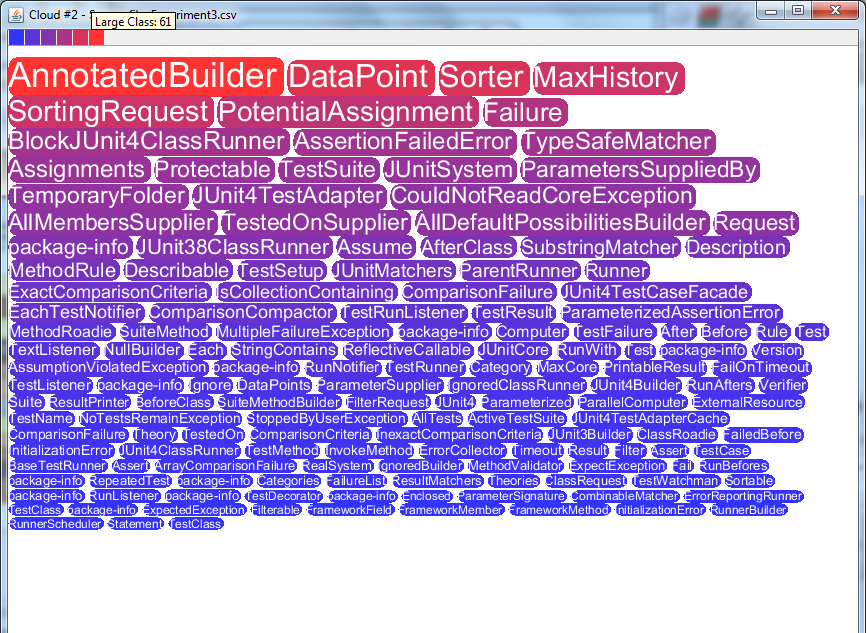
\includegraphics[scale=0.20]{colourbuckets3.png}
	\caption{\textit{Colour gradient between red and blue}}
\end{subfigure}%
\begin{subfigure}{.5\textwidth}
  \centering
  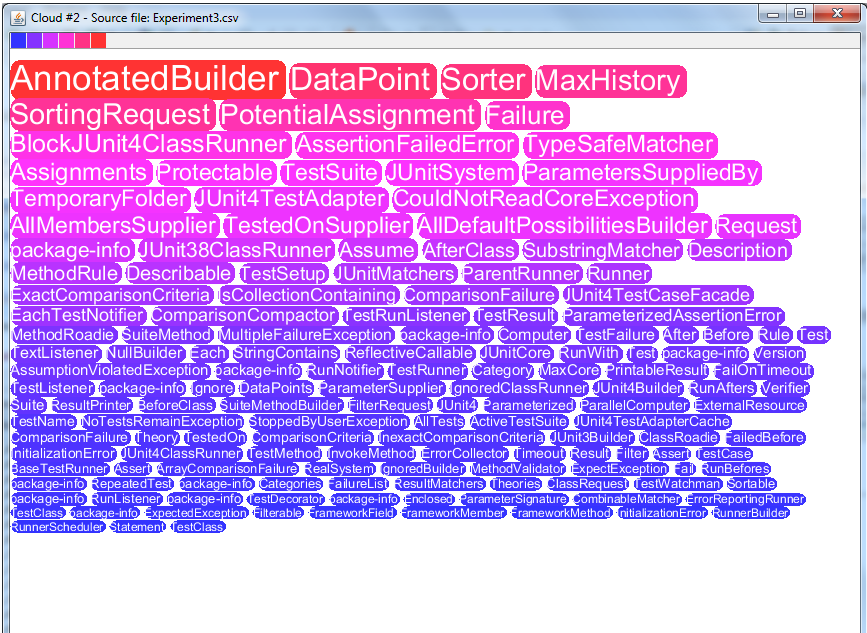
\includegraphics[scale=0.20]{colourbuckets4.png}
  \caption{\textit{Colour wheel between red and blue}}
\end{subfigure}
\begin{subfigure}{\textwidth}
  \centering
  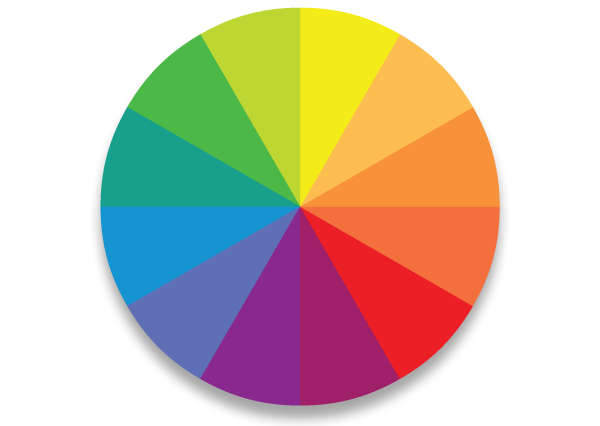
\includegraphics[scale=0.40]{colour_wheel.png}
  \caption{\textit{A colour wheel}}
\end{subfigure}
  \caption{\textit{Displaying continuous data with colour ranges}}
  \label{fig:continuous}
\end{figure}

\paragraph{Visual variable: font colour} The user also has the choice of displaying a more conventional looking tag cloud, with colour mapped to the font rather than the background (see Figure~\vref{fig:fontcolour}).

\begin{figure}[!htb]
  	\centering
   	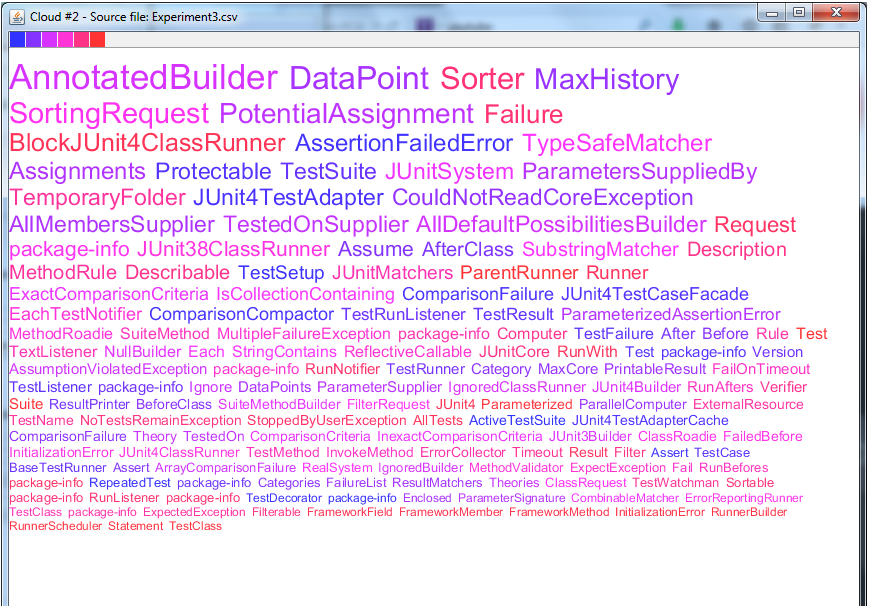
\includegraphics[scale=0.35]{fontcolour.png}
  	\caption{\textit{Colour mapped to the font}}
	\label{fig:fontcolour}
\end{figure}

\paragraph{Visual variable: transparency} The user may map data fields to a visual property which is familiarly used in tag clouds online --- transparency --- see Figure~\vref{fig:transparency}. This can be applied with or without colour.

\begin{figure}[!htb]
\begin{subfigure}{.5\textwidth}
	\centering
	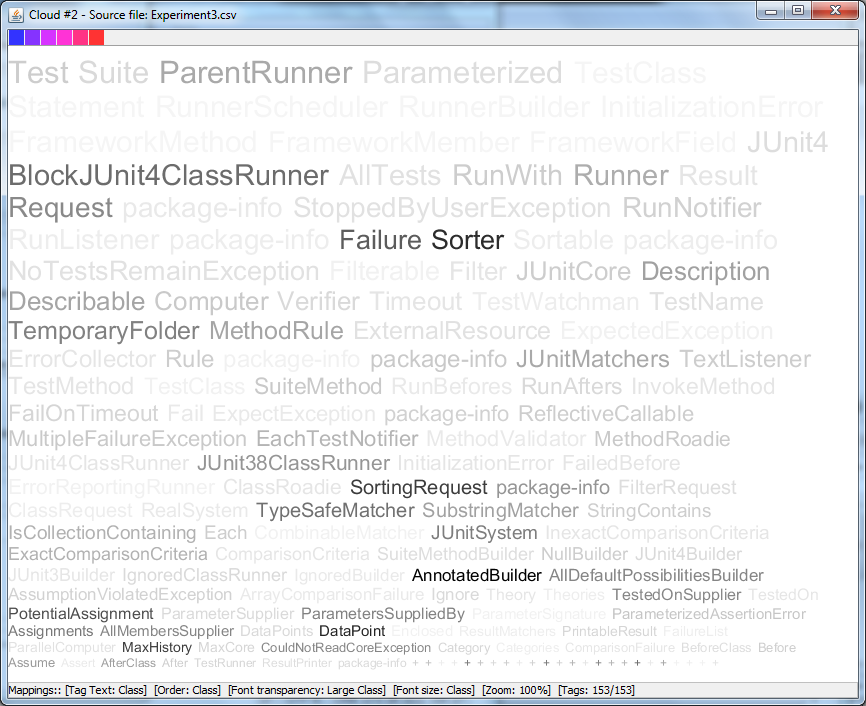
\includegraphics[scale=0.20]{transparency.png}
	\caption{\textit{Without colour applied}}
\end{subfigure}%
\begin{subfigure}{.5\textwidth}
  \centering
  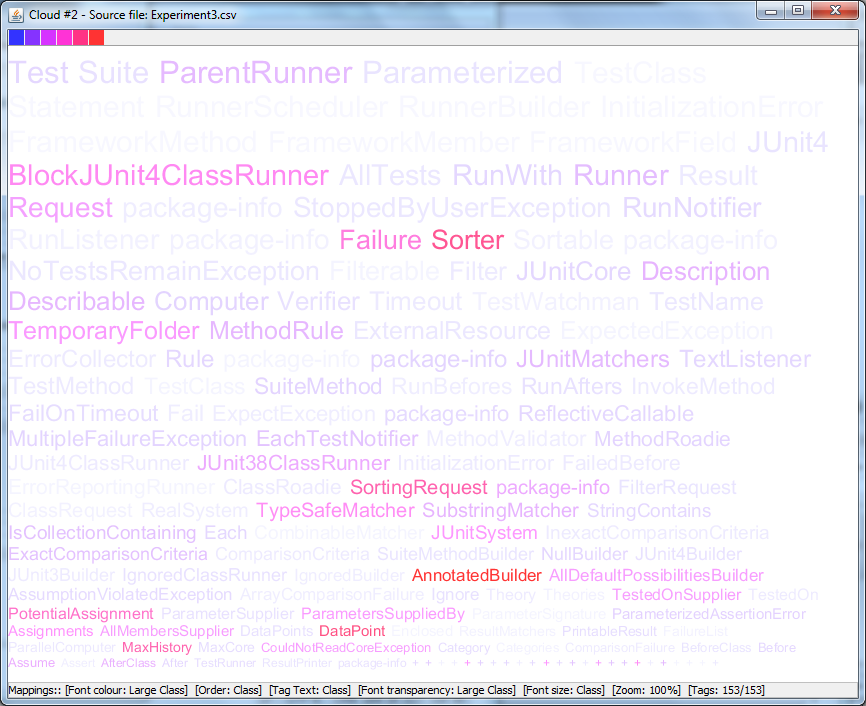
\includegraphics[scale=0.20]{transparency2.png}
  \caption{\textit{With colour applied}}
\end{subfigure}
  	\caption{\textit{Transparency mapping}}
	\label{fig:transparency}
\end{figure}

%\subsection{Bertin's visual variables}

%Chosen mappings are selective and associative. Quantitative issues - comparisons using mouse drags.

\section{Software engineering tasks}\label{sect:softwaretasks}

Taggle includes a number of interactive features to enable rich data exploration. Only the features which were utilised in this research and pertain directly to completing the software engineering tasks outlined in \S\ref{sect:tasktypes} are described in this section. For further information describing features such as relationship highlighting, cloud listeners, sub-clouds and linking, see technical documents: \citet{deaker11, deaker11c}.

\subsection{Filtering textual data}\label{sect:textualdata}

Textual data is an issue with some multi-variate data visualisation techniques such as treemaps or scatterplots because of issues with screen real estate. On the other hand, a tag cloud is designed to include the (often important and identifying) textual data as a key part of the graphic. Software textual data is often in the form of long identifiers such as class or agile story names. Taggle's mouse wheel filtering (used for textual data displayed in the tag, interface shown in Figure~\vref{fig:filtering1}) can be used to dynamically select the portions of the text identifier that the user deems most important and/or maximise the available visualisation space. When the `Tag delimiter' option is selected, the user may filter the text by a particular character by scrolling the mouse wheel (scrolling up filters off leading text while scrolling down filters off trailing text). In Figure~\vref{fig:filtering2} you can see an example of typical software engineering data displaying Java package and class names as the textual identifier in the text with a) showing the original tag text and b) text filtered to two packages above the class name.

\begin{figure}[!htb]
  	\centering
   	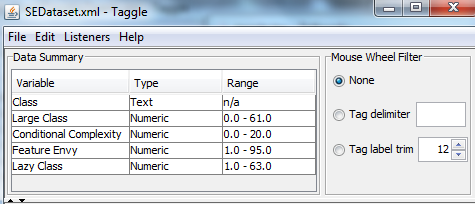
\includegraphics[scale=0.75]{mousefilter.png}
  	\caption{\textit{Mouse filtering interface}}
	\label{fig:filtering1}
\end{figure}

\begin{figure}[!htb]
\begin{subfigure}{\textwidth}
	\centering
	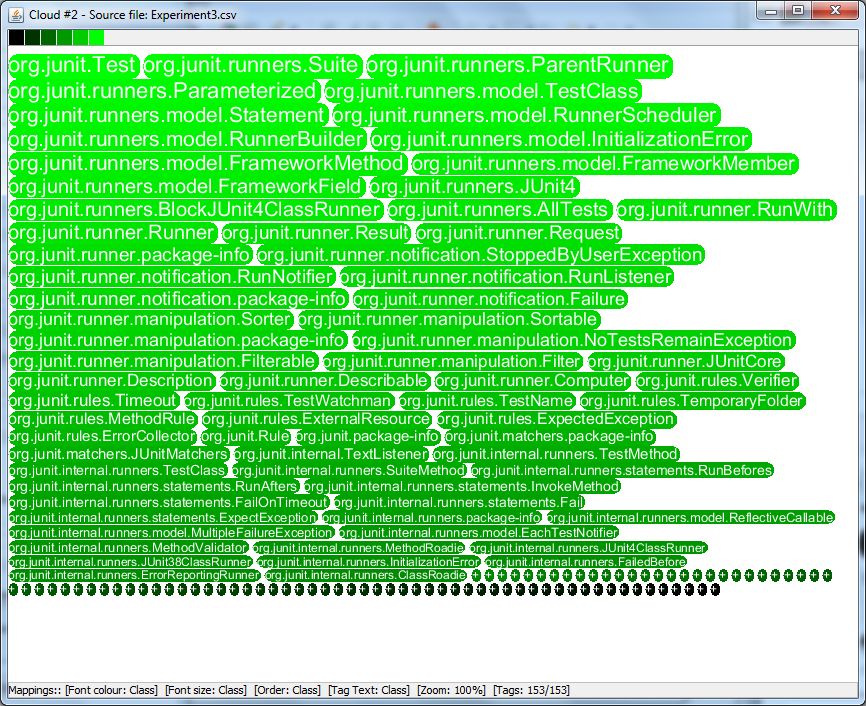
\includegraphics[scale=0.35]{delimiterfilter1.png}
  	\caption{\textit{Original tag text}}
\end{subfigure}
\begin{subfigure}{\textwidth}
 	 \centering
	 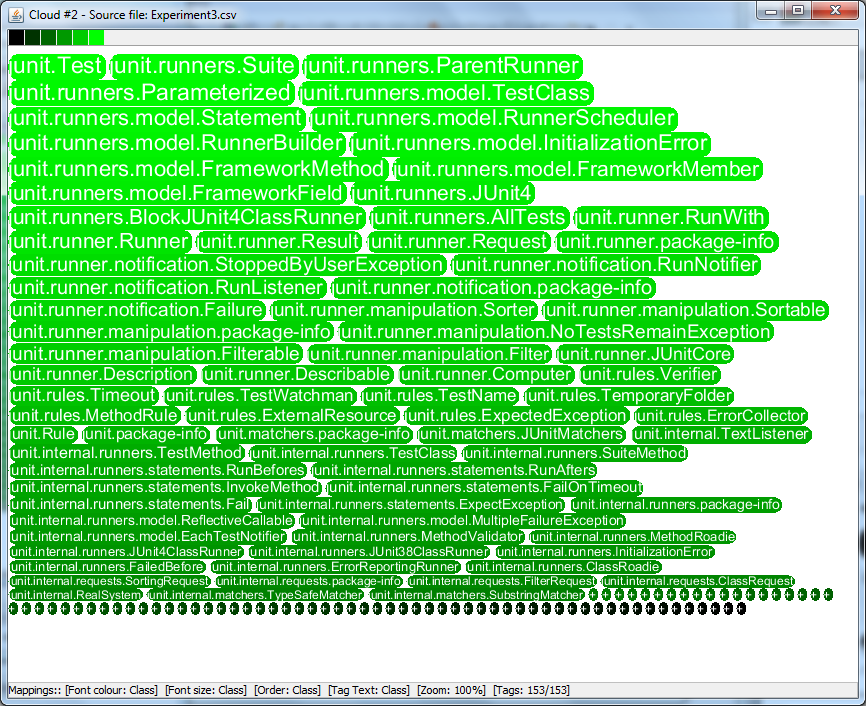
\includegraphics[scale=0.35]{delimiterfilter2.png}
	 \caption{\textit{Filtered on a `.' delimiter}}
\end{subfigure}
  \caption{\textit{Filtering on a character delimiter}}
  \label{fig:filtering2}
\end{figure}

The user also has the option of filtering the text to a fixed number of characters from either the leading or trailing text (Figure~\vref{fig:filtering3}). This has two purposes, to maximise available real estate in the canvas, and to minimise any effect a greater number of characters in a tag may have on user perception. This filter can be used in combination with removing the font size mapping selection, which further minimises bias in eye attention.  

\begin{figure}[!htb]
  	\centering
   	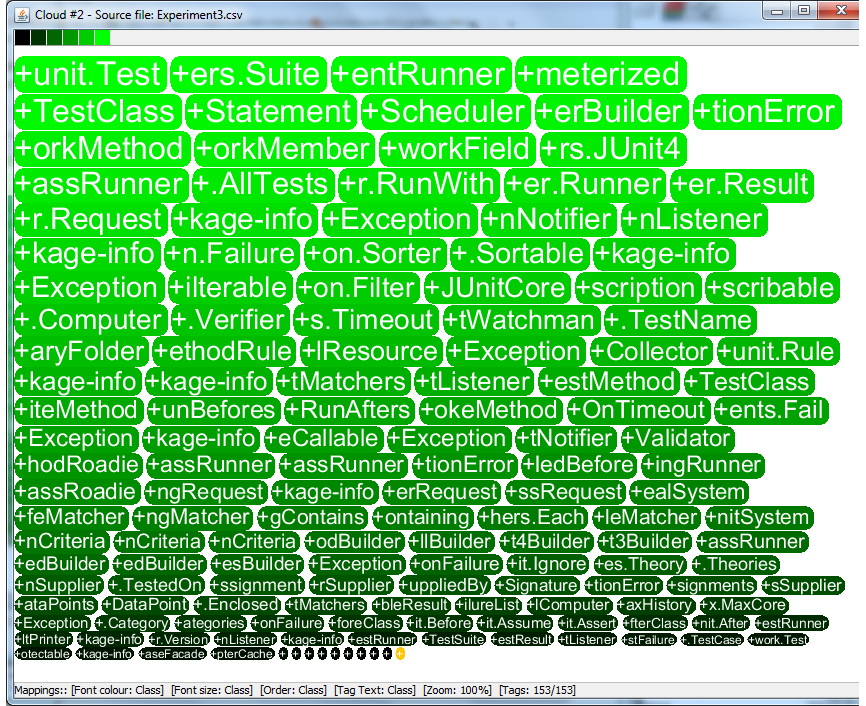
\includegraphics[scale=0.35]{taglabeltrimfilter.png}
  	\caption{\textit{Filtering on a fixed number of characters from the leading text}}
	\label{fig:filtering3}
\end{figure}

\subsection{Dealing with large scale data}

One feature of software engineering datasets is that there is often a large number of data points to contend with, and any potential visualisation tool must provide a mechanism to deal with this. Using the ``Information Seeking Mantra'' \citep{schneiderman96}, we first provide the user with an overview of the dataset (see Figure~\vref{fig:detailsondemand}), and allow additional details to be accessed on demand via a mouse hover. As seen in Figure~\vref{fig:filtering2}, tag labels too long to be displayed on the canvas are minimised into symbols. This has the advantage that they don't disappear from view together, and hovering over the iconified form reveals their details. As the user interacts with the data using filtering and dynamic queries, these symbols are transformed into textual labels as canvas real estate becomes available. 

\begin{figure}[!htb]
  	\centering
   	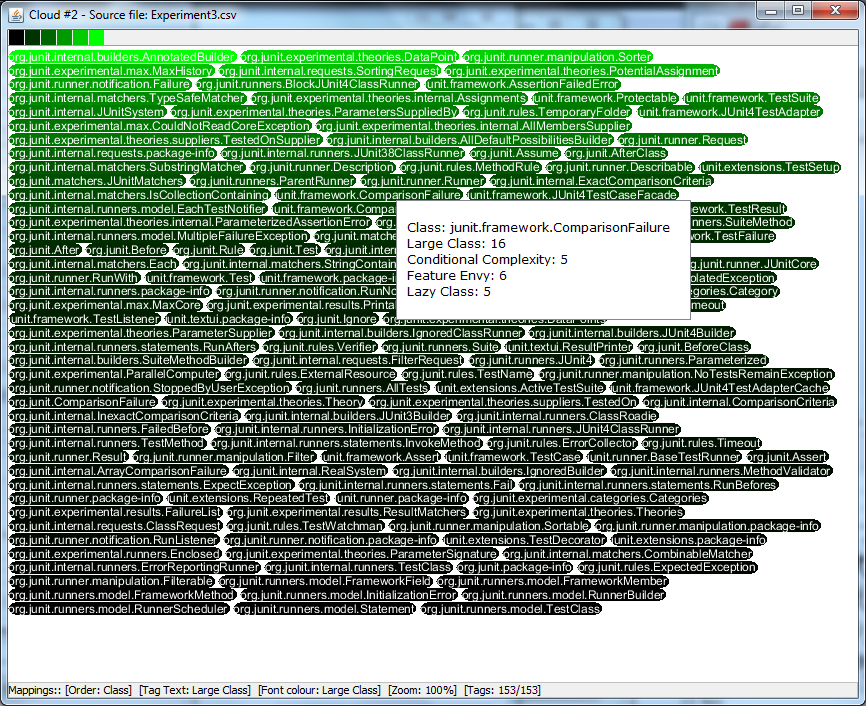
\includegraphics[scale=0.35]{detailsondemand.png}
  	\caption{\textit{Overview first, then details-on-demand}}
	\label{fig:detailsondemand}
\end{figure}

Filtering can be applied to the dataset (Figure~\vref{fig:staticfilter}) to narrow the view as desired, or dynamic querying (Figure~\vref{fig:taggledynamicfilter}) where the user is able to see the tags filtered from display in real time using a range slider. 

\begin{figure}[!htb]
  	\centering
   	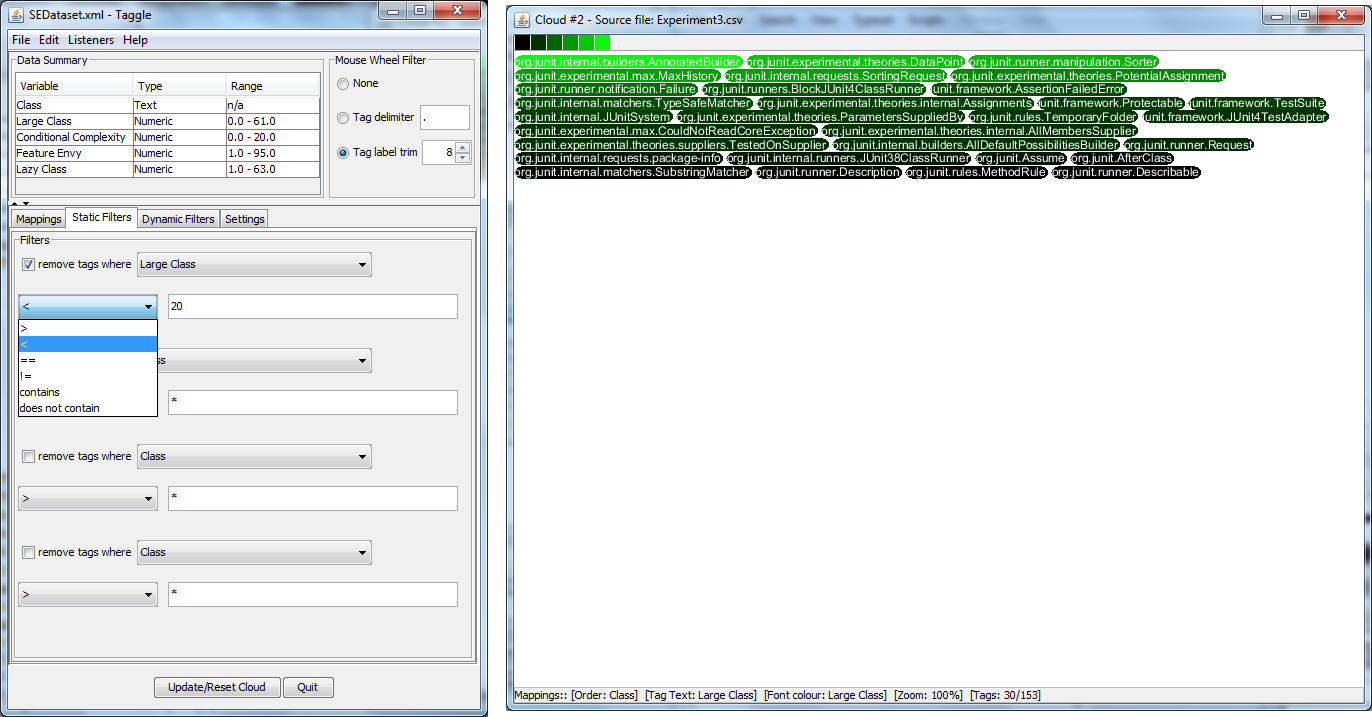
\includegraphics[scale=0.30]{staticfilter.png}
  	\caption{\textit{Applying filtering to the data}}
	\label{fig:staticfilter}
\end{figure}

\begin{figure}[!htb]
  	\centering
   	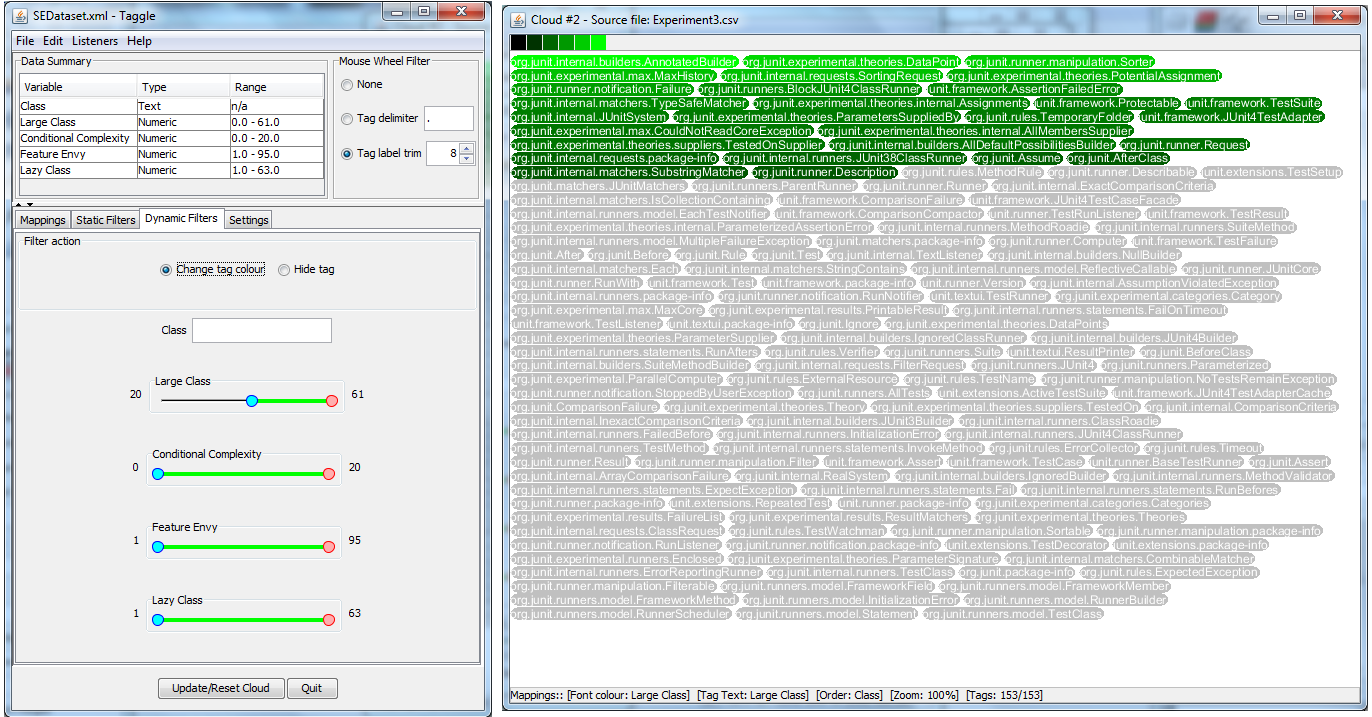
\includegraphics[scale=0.30]{dynamicfilter.png}
  	\caption{\textit{Dynamic querying}}
	\label{fig:taggledynamicfilter}
\end{figure}

It is also possible to display an overview of data while allowing detailed information to be shown simultaneously with a zoom function (Figure~\vref{fig:zoom}). A particular concern using the tag cloud technique is lack of space due to long label lengths, or many labels with a large dataset. In this case the user may apply dynamic mouse wheel filtering and label trimming as detailed in \S\ref{sect:textualdata}.

\begin{figure}[!htb]
  	\centering
   	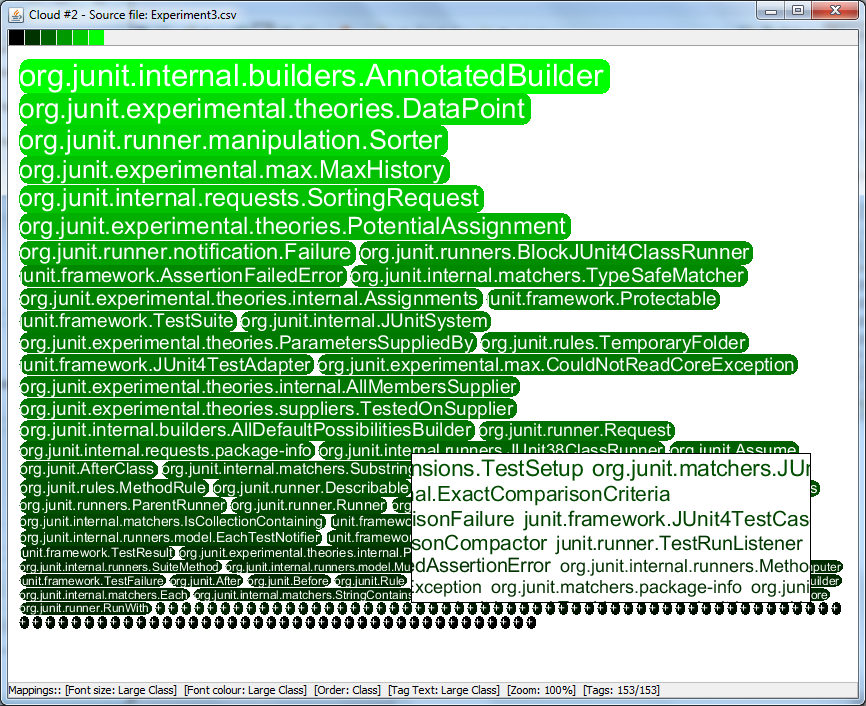
\includegraphics[scale=0.40]{zoom.png}
  	\caption{\textit{Zoom in on a small area}}
	\label{fig:zoom}
\end{figure}

\subsection{Identify similar characteristics of data}

Similar data characteristics can be identified using filtering and details-on-demand. In Figure~\vref{fig:cluster}, a user inspects the classes with a low level of the `lazy class' metric within a software dataset. Using either dynamic queries or details-on-demand on the filtered dataset it is possible to establish that classes with a low level of `lazy class' also have a low level of metric `feature envy' (refer to Chapter~\ref{chap:exp3} for further details regarding this example dataset). Following this kind of filtered inspection, a user might make use of a visual property mapping such as colour to identify a data correlation between the two variables (see \S\ref{sect:datacorrelation}).

\begin{figure}[!htb]
  	\centering
   	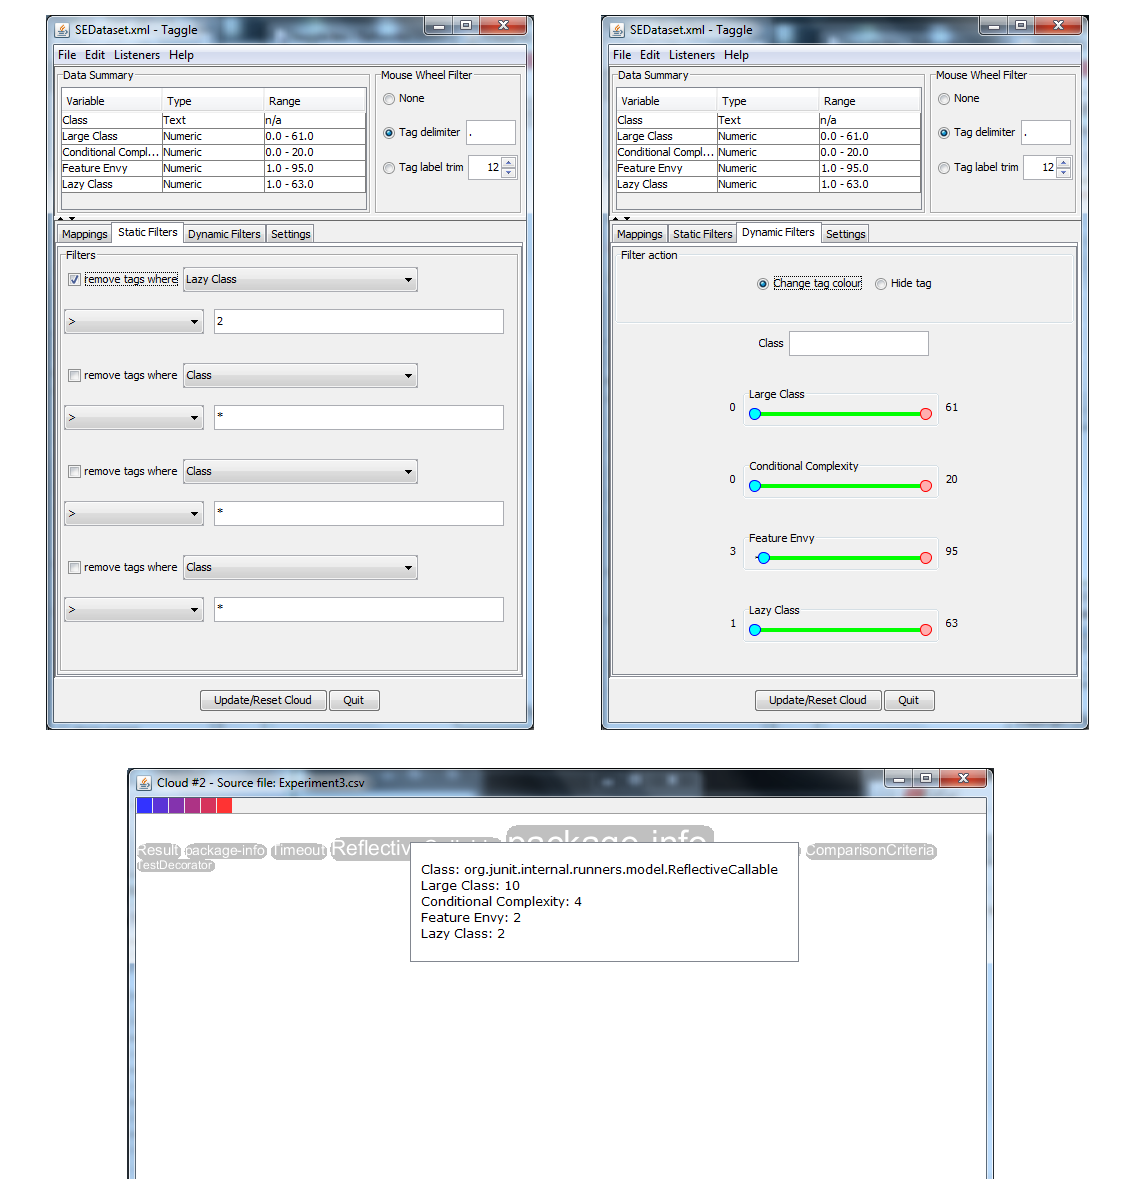
\includegraphics[scale=0.30]{cluster1.png}
  	\caption{\textit{Using filtering to identify similar data characteristics}}
	\label{fig:cluster}
\end{figure}

\subsection{Identifying data distribution}

The distributions of variables in software engineering metric datasets are often heavily skewed (see Figure~\vref{fig:distributions} for some graphical examples of this). In Taggle, colour and order are mapping choices which can be applied to the data in order to highlight data distribution. In Figure~\vref{fig:distribution}, the metric `large class' is being visualised from a software project. To avoid bias in user perception, font size is unmapped and the tag labels have been filtered to a fixed length. The ordering of the tags is arranged in order of the metric in question, from largest value to smallest. A colour gradient between green and black is also mapped to `large class', where black identifies tags which have the lowest levels of `large class', and green shows tags with the highest levels. The distribution of colour across the visualisation shows the user that values of `large class' are skewed towards the lower end as expected. As a user of Taggle, the classes that would now become of interest as possible candidates for refactoring would be the few brightest green tags to the top left.

\begin{figure}[!htb]
  	\centering
   	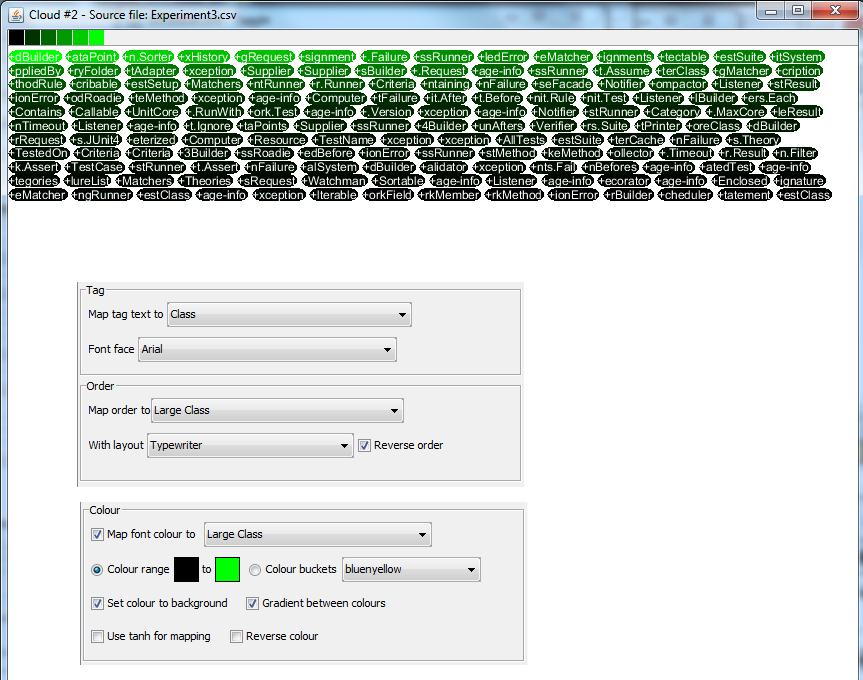
\includegraphics[scale=0.40]{distribution.png}
  	\caption{\textit{Using colour to identify data distribution of the `large class' metric}}
	\label{fig:distribution}
\end{figure}

\subsection{Identify data correlations and outliers}\label{sect:datacorrelation}

Software metric data distributions are typically heavily skewed and may contain outliers. In statistics, outliers are often discarded or ignored during analysis: in software engineering these outliers are often points of interest. In Figure~\vref{fig:correlation}, colour and order are used to investigate a possible correlation between data variables, metrics `lazy class' and `feature envy'. Size and order are dually mapped to `feature envy' while a colour range (blue to red) is mapped to `lazy class'. We see that as the font size becomes smaller, the colour mapping changes gradually from red to blue in a progressive fashion. This is indicative of a correlation between the two variables. There are three data points which have colouring that stands out amongst the rest (classes `Enclosed', `Theory' and `JUnit4TestAdapter'), these points may appear as outliers in the correlation between the data variables. In Figure~\vref{fig:correlation1}, colour is scattered without pattern across the order and font size, no correlation can be seen between variables `conditional complexity' and `feature envy'.

\begin{figure}[!htb]
  	\centering
   	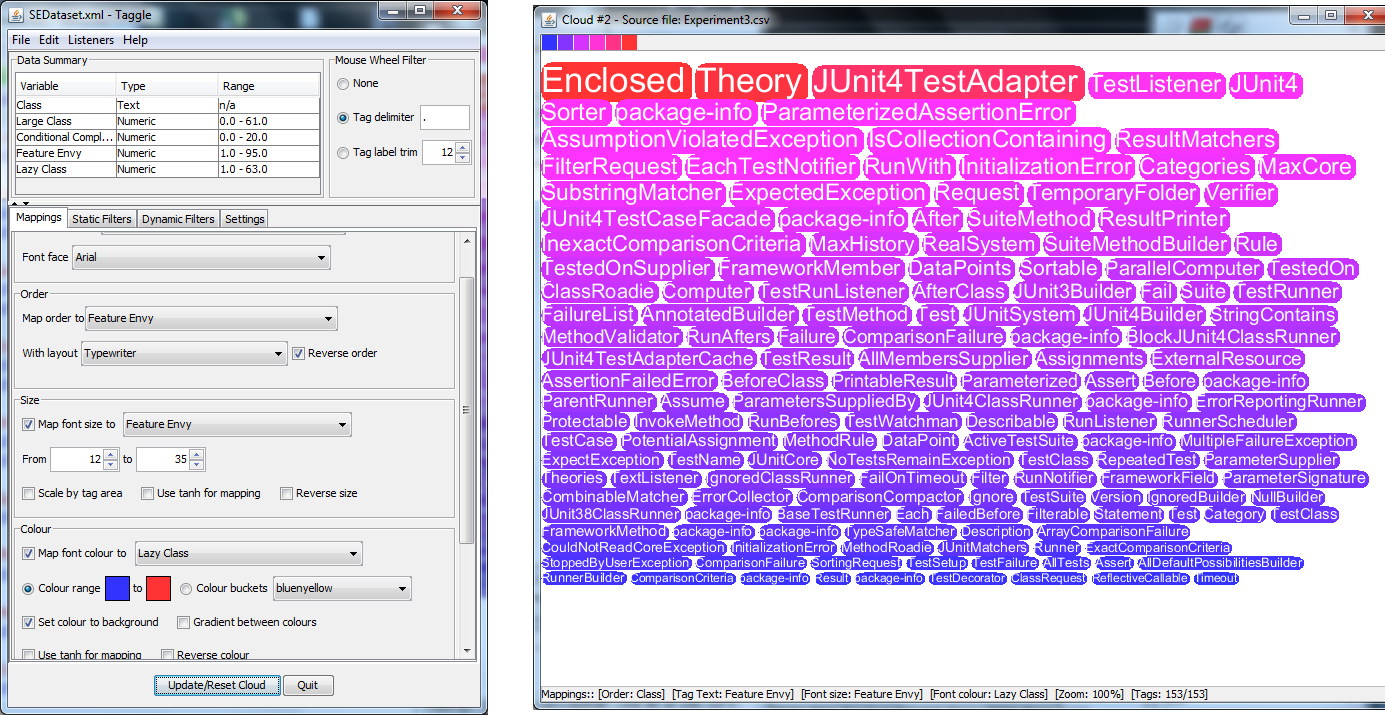
\includegraphics[scale=0.30]{correlation.png}
  	\caption{\textit{Using colour to identify a data correlation and outliers}}
	\label{fig:correlation}
\end{figure}

\begin{figure}[!htb]
  	\centering
   	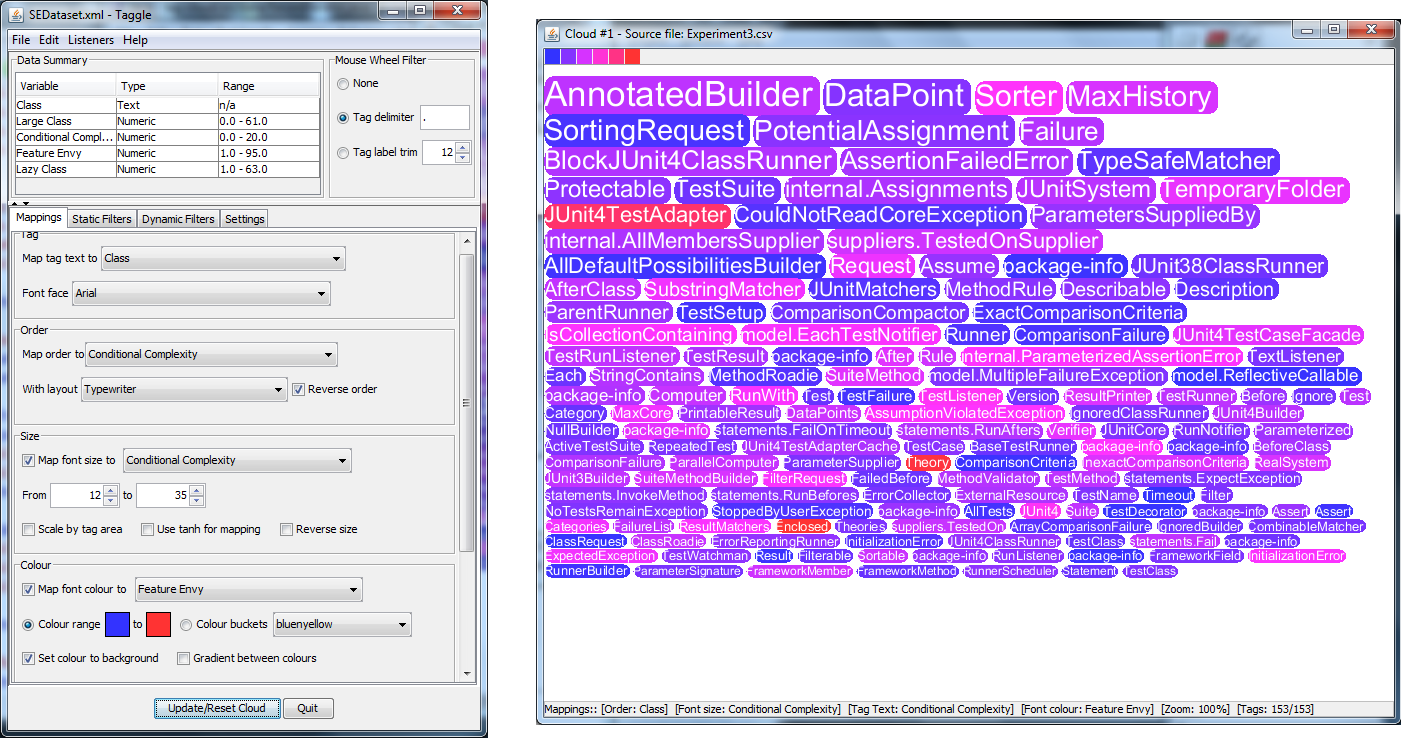
\includegraphics[scale=0.30]{correlation1.png}
  	\caption{\textit{No data correlation between variables}}
	\label{fig:correlation1}
\end{figure}

\subsection{Finding minimum/maximum values}

In software metric analysis, finding classes which hold the minimum or maximum values of a metric is useful for identifying classes that are candidates for refactoring. The order mapping, or a dual mapping of order and font size, are useful for identifying classes in the lower and upper boundaries. In Figure~\vref{fig:minimum1}, `AnnotatedBuilder' and `DataPoint' classes are easily identified as having the highest values of the `conditional complexity' metric when dually mapped to order and font size.

\begin{figure}[!htb]
  	\centering
   	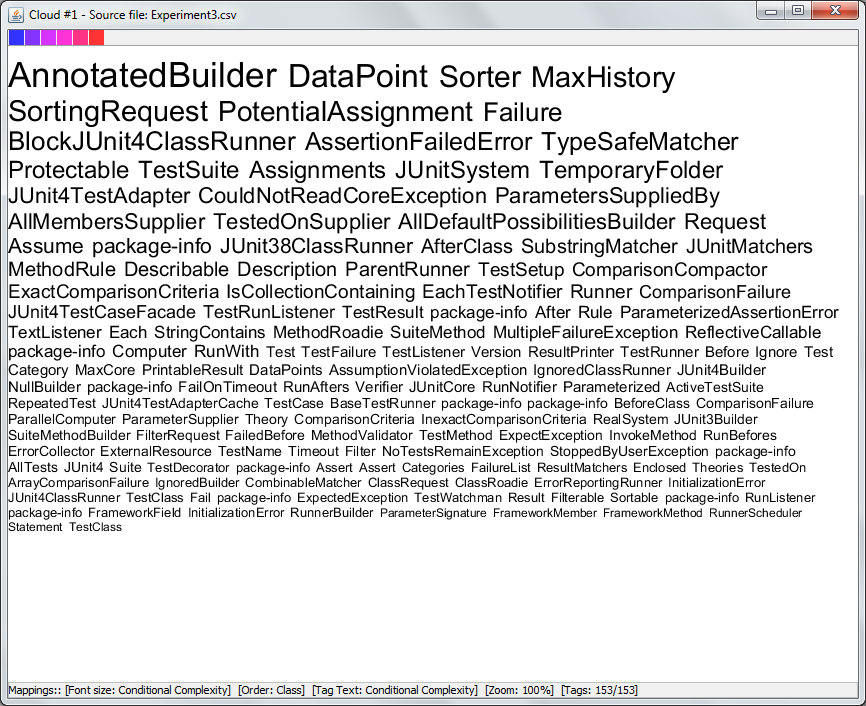
\includegraphics[scale=0.40]{minimum1.png}
  	\caption{\textit{Finding classes with the highest value of a metric using \\dual order and font size mappings}}
	\label{fig:minimum1}
\end{figure}

\subsection{Comparison of data elements}

Comparison of data points is another key task useful in any software engineering or multi-variate dataset. In Figure~\vref{fig:minimum1} font size and order are dually mapped to field `conditional complexity'.  It is obvious for example, that tag `JUnitSystem' has a higher conditional complexity than tag `JUnitMatchers'. When font size and order are not mapped to the same data field it may not be so obvious. Using drag and drop a user may pull out the relevant tags and put them next to one another for easier comparison --- see Figure~\vref{fig:comparison}. Additionally, a user may hover over the tags and view the class metric information in the pop-up details-on-demand for comparison.

\begin{figure}[!htb]
  	\centering
   	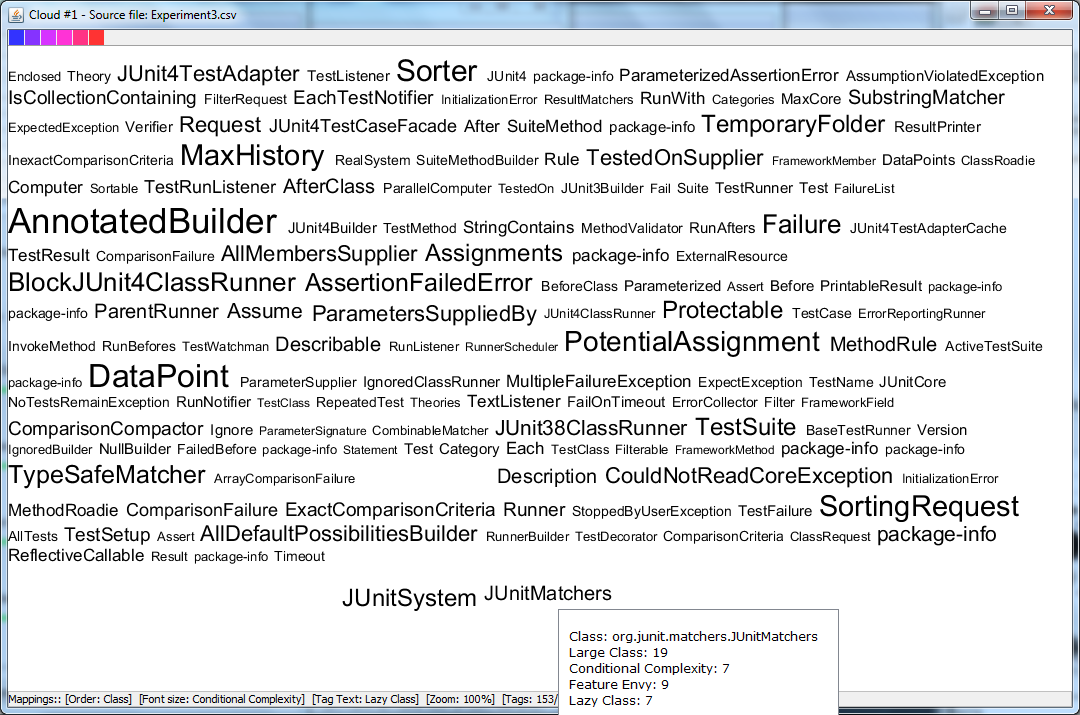
\includegraphics[scale=0.35]{comparison.png}
  	\caption{\textit{Comparison of `JUnitSystem' and `JUnitMatchers'}}
	\label{fig:comparison}
\end{figure}

\section{Summary and discussion}

In this chapter, we introduced the tag cloud visualisation tool Taggle. This tool was inherited from previous research and extensively modified to create a stable system able to explore software quality metrics and other more general multi-variate data. Most notably, a variety of implementation changes were made as a result of considering design aspects from software engineering and tag cloud visual variable analysis (Chapter~\ref{chap:tagcloud}) as well as improvements generated from a heuristic evaluation by domain experts (Chapter~\ref{chap:heuristiceval}).

Data can be gathered from a variety of sources and then converted (through XML transform or conversion utility) into a special Taggle XML format. This XML file is then input into Taggle through the user interface, where the user can view generated tag clouds and customise the visual property mappings as they explore the dataset. Interface and visual encoding design choices such as the visual properties included, constraints and options for each property, and filtering selections were made with respect to the software engineering and design considerations listed in previous chapters. Some choices, such as the data summary screen and categorical data options, were incorporated by request during the heuristic evaluation.

In Chapter~\ref{chap:tagcloud}, a list of tasks was presented that represented meaningful ways users could interact with software data. These included tasks from data mining task types --- clustering, summarising,  associating and classifying --- and involved activities such as identifying similar data characteristics, distribution and correlations. In \S\ref{sect:softwaretasks}, we showed how a user could interact with a sample software engineering dataset to complete each task using the system. Taggle's design was intended to cope specifically with the challenges of software engineering datasets, by using appropriate visual mappings available in tag clouds to render the data.

% ------------------------------------------------------------------------


%%% Local Variables: 
%%% mode: latex
%%% TeX-master: "../thesis"
%%% End: 
